\mode*

\begin{frame}[fragile]{Que fait ce programme ?}
  \begin{tikzpicture}
    \fill[alertColor!20, rounded corners] (4,6.52) rectangle (6.4,6.82);
    \draw[alertColor, thick] (4.1,6.67) -- (6.3,6.67);

    \fill[structure!20, rounded corners] (3.5,3.5) rectangle (8.5,4.15);
    \draw[structure] (11,3.85) node{//$T_{reader}$};

    \fill[exampleColor!20, rounded corners] (5.1,1.85) rectangle (8.5,2.15);
    \draw[exampleColor] (11,2) node{//$T_{writer}$};
    \draw (5,4.85) node{\begin{minipage}{5cm}\begin{lstlisting}[numbers=none]
class Counter {
  private int value=0;
  public synchronized void increment() {
    ++value;
  }
  public synchronized int get() {
    return value;
  }

  public static void main(String[] args) {
    var counter = new Counter();
    
    new Thread(() -> {
      while(counter.get()==0);
      System.out.println("done");
    }).start();
    
    Thread.sleep(250);
   
    new Thread(counter::increment).start();
  }
}
\end{lstlisting}\end{minipage}};
  \end{tikzpicture}
  
  \vspace{-5mm}
\begin{citing}
\jitem \lstinline{tp1/Volatile.java}
\end{citing}
\end{frame}

\begin{frame}[fragile]{Quels affichages sont possibles ?}
  \vspace{-3mm}
  \begin{tikzpicture}
    \fill[structure!20, rounded corners] (4,5.85) rectangle (6.5,6.5);
    \fill[structure!20, rounded corners] (3.5,4.85) rectangle (8.3,5.2);
    \fill[structure!20, rounded corners] (3.5,3.85) rectangle (9.9,4.2);
    \draw (5,4.85) node{\begin{minipage}{5cm}\begin{lstlisting}[numbers=none]
class Optimizations {
  static int sum = 0;
  static int i = 0;
  public static void main(String args[]) {
    new Thread(() -> {
      for(i=1; i<2; i++) sum+=i;
    }).start();
    new Thread(() -> {
      if(sum != 0) System.out.println(i);
    }).start();
  }
}
\end{lstlisting}\end{minipage}};
  \end{tikzpicture}
  \pause
    \vspace{-2mm}
  \begin{block}{Compilateur et JVM : respect de la sémantique séquentielle}
    \vspace{-3mm}
    \begin{minipage}{.35\textwidth}
    \begin{lstlisting}[numbers=none]
for(i=1; i<2; i++)
  sum+=i;

\end{lstlisting}
    \end{minipage}
    \pause
    \hspace{\fill}
    \begin{minipage}{.2\textwidth}
    \begin{lstlisting}[numbers=none]
i=1;
sum=1;
i=2;
    \end{lstlisting}
    \end{minipage}
    \hspace{\fill}
    \pause
    \begin{minipage}{.2\textwidth}
    \begin{lstlisting}[numbers=none]
      
sum=1;
i=2;
    \end{lstlisting}
    \end{minipage}
  \end{block}

    \vspace{-2mm}
\pause
  \begin{exampleblock}{Mot-clé \lstinline{volatile int x;}}
    \begin{itemize}
    \item Pas d'optimisation qui change la position d'une opération sur $x$
    \end{itemize}
  \end{exampleblock}
\end{frame}

\begin{frame}[fragile]{Cohérence de cache}
  \begin{block}{Architectures UMA (Uniform Memory Access)}
    \begin{center}
      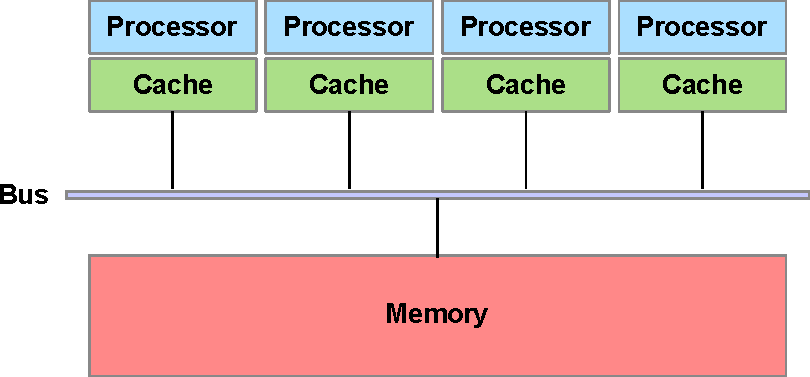
\includegraphics[height=2cm]{uma}
    \end{center}
  \end{block}
  \begin{exampleblock}{Mot-clé \lstinline{volatile int x;} (depuis Java 5)}
    \begin{itemize}
    \item Tout le cache est invalidé \structure{avant chaque lecture}  de $x$
    \item Tout le cache est invalidé \structure{après chaque écriture} de $x$
    \item Le cache n'est pas invalidé \structure{pendant} une lecture ou écriture de $x$ $^\star$
    \end{itemize}
  \end{exampleblock}
  \begin{alertblock}{Attention}
    \begin{itemize}
    \item Une invalidation de cache est très inefficace !
    \end{itemize}
  \end{alertblock}

\vfill

\fontsize{4}{4}\selectfont{ $^\star$ \href{https://docs.oracle.com/javase/specs/jls/se7/html/jls-17.html#jls-17.7}{(§17.7)} \it Implementations of the Java Virtual Machine are \alert{encouraged} to avoid splitting 64-bit values where possible. Programmers are encouraged to declare shared 64-bit values as volatile or synchronize their programs correctly to avoid possible complications.}

\end{frame}


\begin{frame}{Échelles de temps}
   \begin{center}
      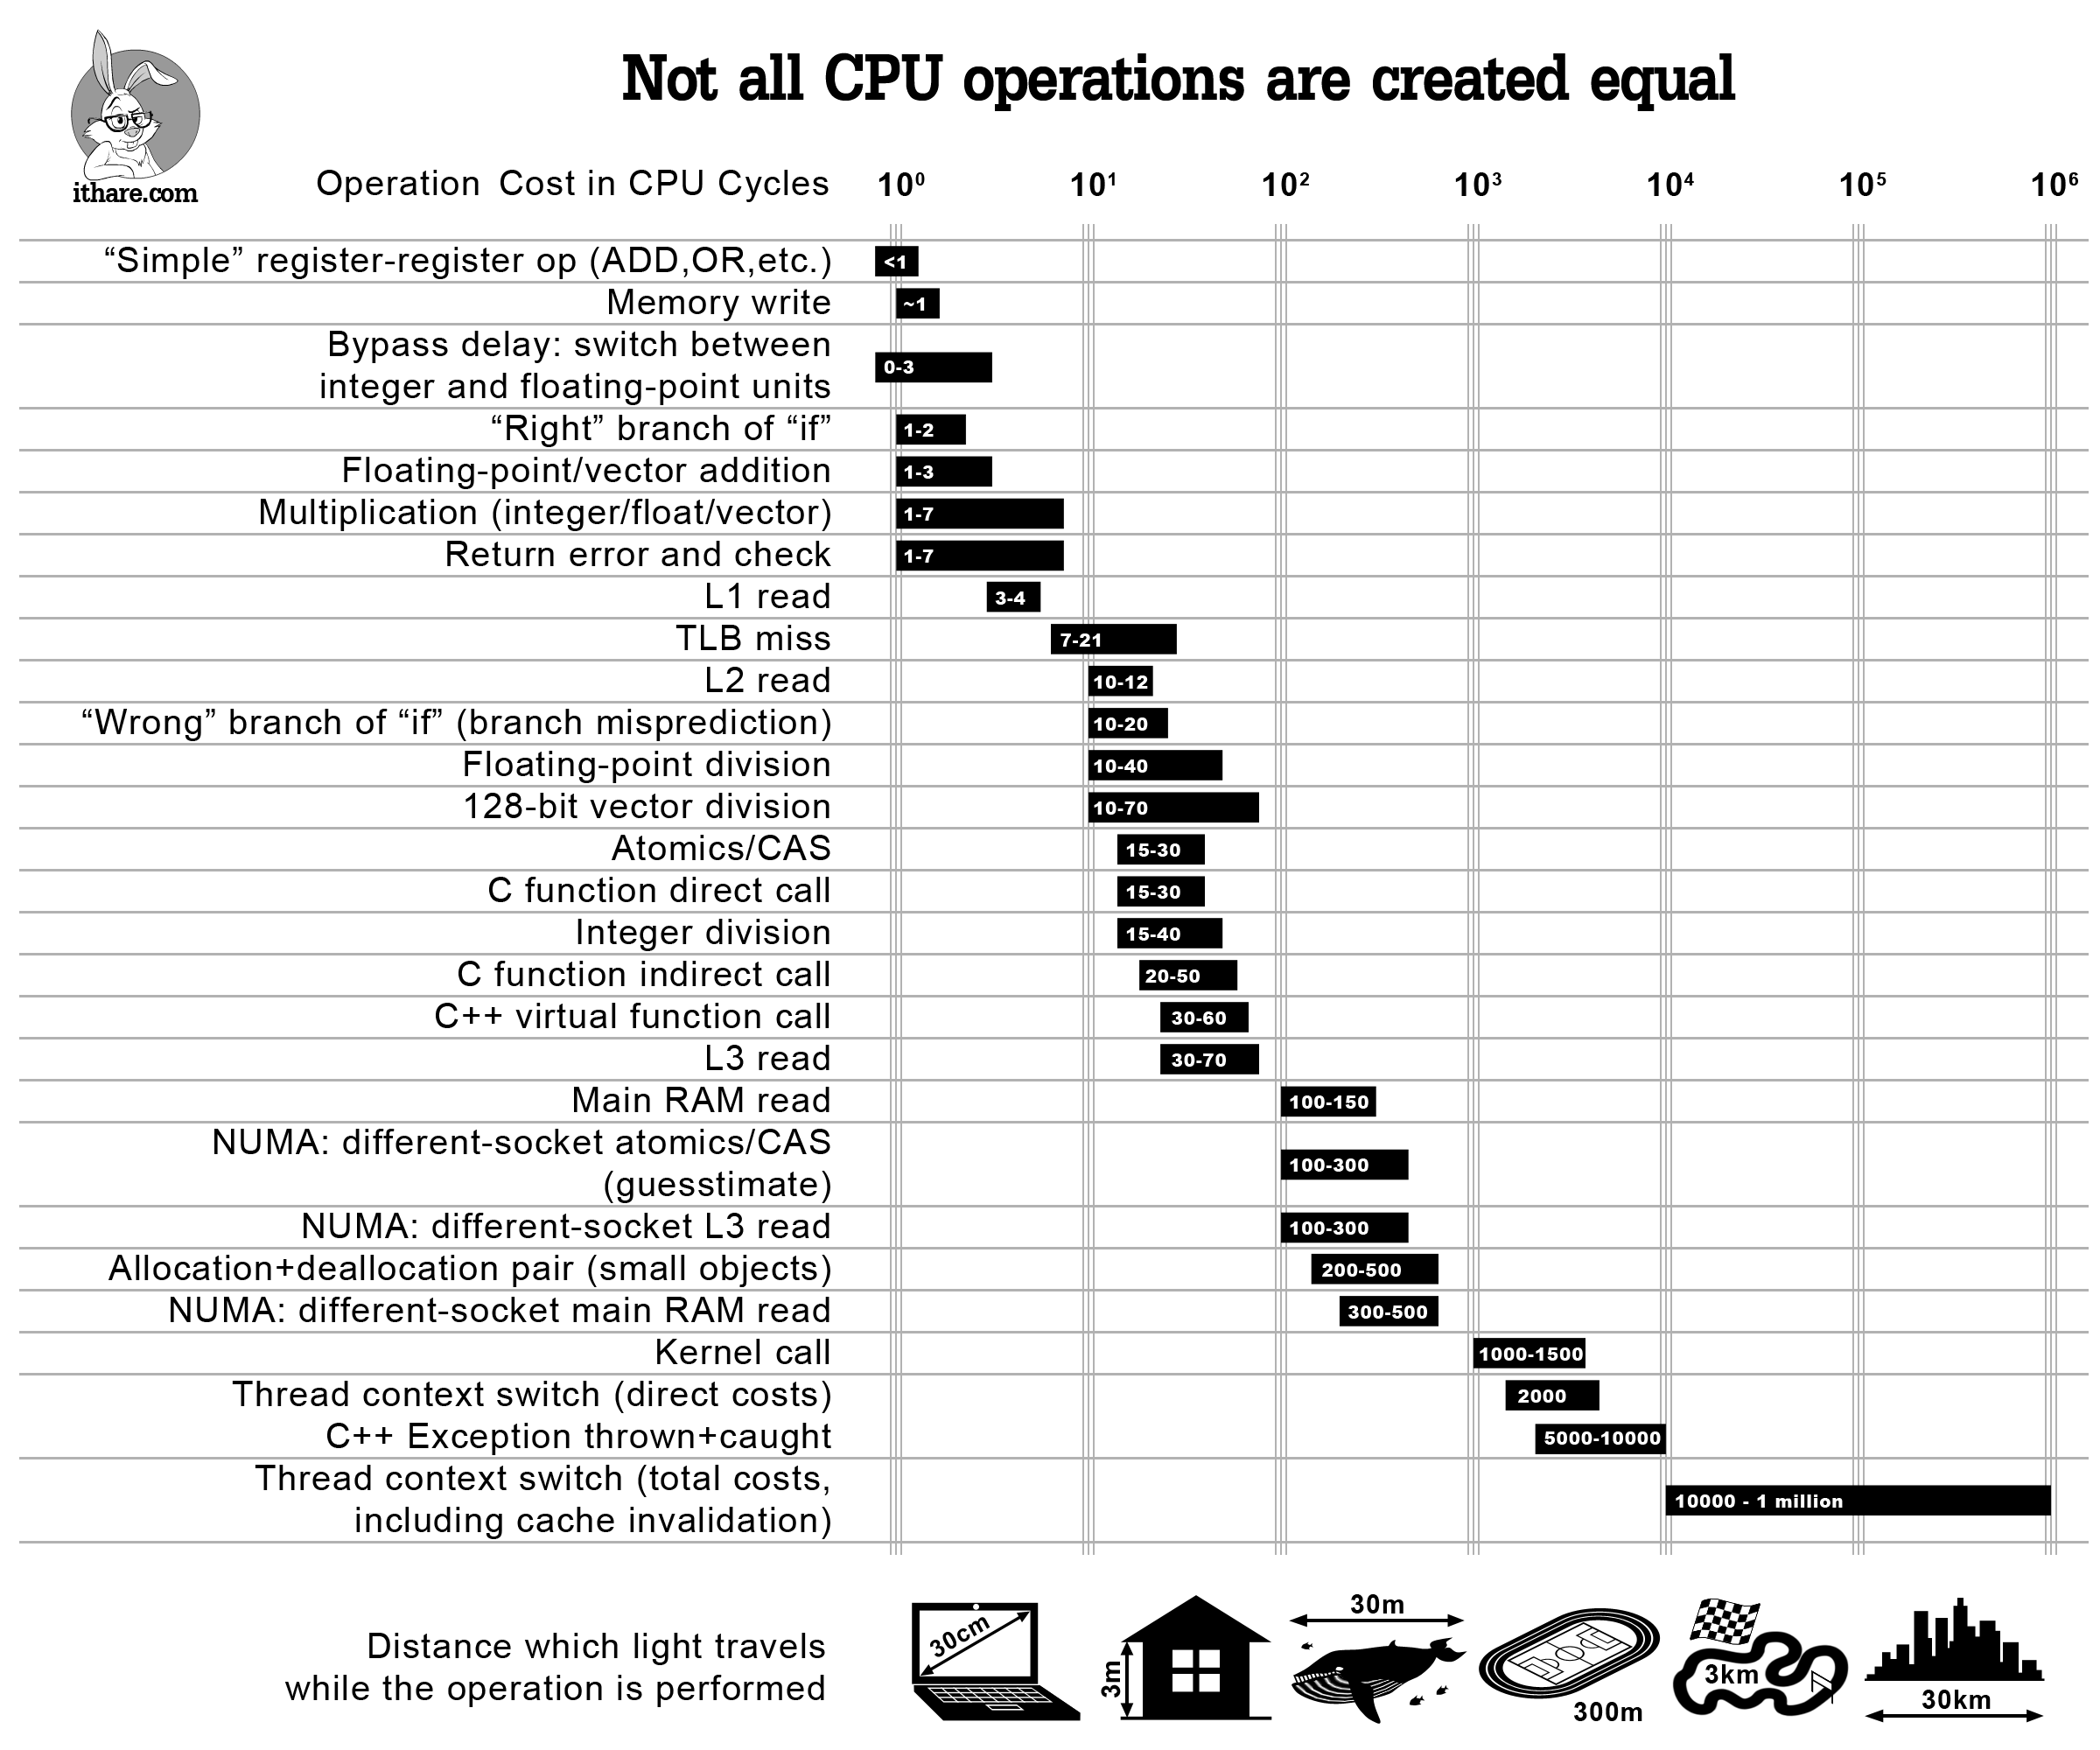
\includegraphics[width=9cm]{time}\\
   \end{center}
\end{frame}


\begin{frame}[fragile]{Modèle de mémoire en Java}
  \begin{block}{Le mot-clé \lstinline{volatile} en Java}
    \begin{itemize}
    \item Les variables \lstinline{volatile} sont linéarisables
    \item Gestion par le système
      \begin{itemize}
      \item Limite les optimisations du compilateur
      \item Limite l'utilisation des caches
      \end{itemize}
    \end{itemize}
  \end{block}
\vfill
  \begin{alertblock}{Toute variable doit être :}
    \begin{itemize}
    \item soit déclarée \lstinline{final}
    \item soit déclarée \lstinline{volatile}
    \item soit uniquement accédée séquentiellement
      \begin{itemize}
      \item exemple des variables locales
      \item par exemple en section critique
      \item lectures et écritures ordonnées par ``happened before''
      \end{itemize}
    \end{itemize}
  \end{alertblock}
\vfill
\begin{citing}
\item \href{https://docs.oracle.com/javase/specs/jls/se7/html/jls-17.html#jls-17.4}{Voir la spécification officielle de la JVM, chapitre 17.4}
\end{citing}
\end{frame}


\begin{frame}{La relation ``happened before'' (ordre causal)}
  $e\mapsto e'$ si l'une des conditions s'applique :    
  \begin{itemize}
  \item \structure{Ordre de programme :} le même thread produit $e$ puis $e'$
  \item \structure{Ordre de synchronisation :} ordre total sur un sous-ensemble d'actions
  \begin{itemize}
    \item Entrée et sortie d'un block \lstinline{synchronized} ;
    \item Lecture et écriture d'une variable \lstinline{volatile} ;
    \item Lancement d'un thread $\mapsto$ première action du thread
    \item $t.interrupt() \mapsto$ détection de l'interruption 
      \begin{itemize}
      \item \lstinline{throw InterruptedException}, \lstinline{interrupted()} ou \lstinline{isInterrupted()}
      \end{itemize}
    \item Dernière action d'un thread $\mapsto$ détection de terminaison
      \begin{itemize}
      \item $t.join()$ ou $t.isAlive()$
      \end{itemize}
    \item Écriture d'une valeur par défaut $\mapsto$ première action d'un thread
  \end{itemize}
  \item \structure{Vie d'un objet :} $e$ est la fin du constructeur et $e'$ l'appel de \lstinline{finalizer}.
  \item \structure{Transitivité :} $\exists e'', e\mapsto e'' \mapsto e'$
  \end{itemize}
  \begin{alertblock}{Happened before consistency pour une variable}
  \begin{itemize}
  \item \alert{Si les seules opérations concurrentes sont des lectures,}
  \item alors chaque lecture retourne la dernière valeur écrite
  \end{itemize}
  \end{alertblock}
\end{frame}

\begin{frame}[fragile]{Exemple (schématique) }
  \begin{tikzpicture}
    \fill<2->[alertColor!20, rounded corners] (3.1,6.85) rectangle (7.5,7.15);
    \fill<2->[alertColor!20, rounded corners] (3.55,4.85) rectangle (6.2,5.15);
    \fill<2->[alertColor!20, rounded corners] (4.5,3.2) rectangle (6.3,3.5);
    \draw (5,5) node{\begin{minipage}{5cm}\begin{lstlisting}[numbers=none]
  class Future<T> {


    final Callable<T> task;
    volatile boolean isDone = false;
    T value = null;


    void init() { // par thread du thread pool
      value = task.call();
      isDone = true;
    }


    T get() { // par autre thread
      while(!isDone);
      return value;
    }


  }
  \end{lstlisting}\end{minipage}
  };

    \draw<3->[|->, structure, thick, rounded corners] (6.5,5.2) -- (6.5,5) -- (6.2,5);
    \draw<3->[structure] (6.5,4.65) node[right] {Ordre de programme};
    \draw<2->[|->, alertColor, thick, rounded corners] (3.5,5) -- (3,5) -- (3,3.3) -- (3.5,3.3);
    \draw<2->[alertColor] (3.1,4.25) node[right]{Ordre de synchronisation};
    \draw<3->[|->, structure, thick, rounded corners] (6.3,3.35) -- (6.5,3.35) -- (6.5,3) -- (6,3);
    \draw<3->[structure] (6.15,2.7) node {Ordre de programme};
    \draw<4>[|->, exampleColor, thick, rounded corners] (7.5,5.3) -- (10,5.3) -- (10,3) -- (6.5,3);
    \draw<4>[exampleColor] (10,4.15) node[right] {Transitivité};

\end{tikzpicture}
\end{frame}

\begin{frame}[fragile]{Retour sur le calcul de $\pi$}
  \begin{tikzpicture}
    \fill[structure!20, rounded corners] (6.7,6.2) rectangle (8.5,6.5);
    \fill[alertColor!20, rounded corners] (6.9,3.2) rectangle (8.6,3.5);
    \fill[structure!20, rounded corners] (8.05,2.52) rectangle (9.8,2.82);

    \draw[|->, alertColor, thick, rounded corners] (8.7,6.35) -- (10,6.35) -- (10,3.35) -- (8.7,3.35);
    \draw[|->, structure , thick]                  (8.4,3.1) -- (8.4,2.92);
    
    \draw (5,5) node{\begin{minipage}{5cm}\begin{lstlisting}[numbers=none]
public class PiMonteCarlo implements Runnable {
  private int result = 0;
  public void run() {
    for(int i = 0; i<nbIterations; i++) {
      double x = random.nextDouble();
      double y = random.nextDouble();
      if(x*x + y*y < 1) result++;
    }
  }
  static int experiment() {
    for(int i = 0; i<nbThreads; i++) {
      tasks[i] = new PiMonteCarlo();
      threads[i] = new Thread(tasks[i]);
    }
    for(var t : threads) t.start();
    for(var t : threads) t.join();
    int result = 0;
    for(var t : tasks) result+=t.result;
    return result;
  }
}
\end{lstlisting}\end{minipage}};
  \end{tikzpicture}
\end{frame}



\begin{frame}[fragile]{Modèle de mémoire en C++}
\vfill
  \begin{block}{Le mot-clé \lstinline{volatile} en C++}
    \begin{itemize}
    \item Limite les optimisations du compilateur
    \item \alert{Ne place pas les barrières de mémoire}
    \end{itemize}
  \end{block}
\vfill
  \begin{block}{Barrières de mémoire en C++}
      \begin{itemize}
      \item \lstinline{void std::atomic_thread_fence( std::memory_order order )}
      \item Choix de synchronisation read/write, write/read...
        \begin{itemize}
        \item Seulement \lstinline{memory_order_seq_cst} chez Intel
        \end{itemize}
      \end{itemize}
  \begin{shadequote}{Phil Karlton}
    There are only two hard things in Computer Science: \\cache invalidation and naming things.
  \end{shadequote}
  \end{block}

\vspace{-3mm}
\begin{alertblock}{C++ Core Guidelines}
    \begin{description}
    \item[CP.8] \href{https://isocpp.github.io/CppCoreGuidelines/CppCoreGuidelines#Rconc-volatile}{Don’t try to use \lstinline{volatile} for synchronization}
    \end{description}
    \begin{itemize}
    \item Utiliser \lstinline{template <class T> struct std::atomic}
    \end{itemize}
  \end{alertblock}
\vspace{-1mm}
  \begin{citing}
  \item Tutoriel de Ori Lahav sur les modèles de mémoire en C++
  \end{citing}
\end{frame}


\begin{frame}[fragile]{Limite de \lstinline{volatile} : les tableaux}
  \begin{exampleblock}{Tableaux volatiles}
    \begin{lstlisting}[numbers=none]
volatile int array[];
array = new int[10];          // volatile
array[5] = 3;                 // pas volatile
    \end{lstlisting}    
  \end{exampleblock}
  \pause
  \begin{alertblock}{Première solution}
    \begin{lstlisting}[numbers=none]
class VolatileInt{public volatile int x=0;}
VolatileInt array[] = new VolatileInt[10];
array[5] = new VolatileInt(); // pas volatile
array[5].x = 3;               // volatile
    \end{lstlisting}
  \end{alertblock}
  \pause
  \begin{block}{Meilleure solution: \lstinline{java.util.concurrent.atomic.AtomicIntegerArray}}
    \begin{lstlisting}[numbers=none]
AtomicIntegerArray array = new AtomicIntegerArray(10);
array.set(5, 3);              // volatile
    \end{lstlisting}
  \end{block}    
\end{frame}


\begin{frame}[fragile]{Le compteur bloquant}
\begin{enumerate}
\item Si beaucoup de lectures :

  \begin{tikzpicture}
    \fill[alertColor!20, rounded corners] (4.3,5.7) rectangle (5.8,6);
    \draw (5,4.85) node{\begin{minipage}{5cm}\begin{lstlisting}[numbers=none]
class Counter {
  private volatile int value=0;
  public synchronized void increment() {
    ++value;
  }
  public int get() {
    return value;
  }
}
\end{lstlisting}\end{minipage}};
  \end{tikzpicture}
\item Si plus d'incrémentations que de lectures :

\begin{tikzpicture}
    \fill[alertColor!20, rounded corners] (4,4.35) rectangle (6.4,4.65);
    \draw (5,4.85) node{\begin{minipage}{5cm}\begin{lstlisting}[numbers=none]
class Counter {
  private int value=0;
  public synchronized void increment() {
    ++value;
  }
  public synchronized int get() {
    return value;
  }
}
\end{lstlisting}\end{minipage}};
  \end{tikzpicture}
\end{enumerate}
\end{frame}


\mode<all>
